\documentclass{astroedu-lab}

\begin{document}

\pagestyle{plain}

\begin{problem}{\huge Лабораторная работа 4.7.2\\\\Эффект Поккельса\\\\Выполнил Жданов Елисей Б01-205}

\section{Цель работы:}

1) Исследовать интерференцию рассеянного света, прошедшего кристалл

2) Наблюдать изменение характера поляризации света при наложении на кристалл электрического поля

\section{Оборудование:}

1) Гелий-неоновый лазер

2) Поляризатор

3) Кристалл ниобата лития

4) Матовая пластинка

5) Экран

6) Источник высоковольтного переменного и постоянного напряжения

7) Фотодиод

8) Осциллограф

9) Линейка

\section{Теоретическая справка}

Эффектом Поккельса называется изменение показателя преломления света в кристалле под действием электрического поля, причём это изменение пропорционально напряжённости электрического поля. Вследствие эффекта Поккельса в кристалле либо появляется двойное лучепреломление, либо меняется его величина (если кристалл был двулучепреломляющим в отсутствие поля), либо, как в данной работе, одноосный кристалл становится двуосным.

%Изменение показателя преломления кристаллов под действием внешнего электрического поля происходит за счёт анизотропных свойств кристаллов. Под действием постоянного электрического поля электроны смещаются в сторону того или иного иона (в случае кристалла ниобата лития $LiNbO_3$ - это ион Li или Nb), при этом меняется поляризуемость среды и связанный с ней показатель преломления. В первом приближении это изменение линейно относительно внешнего электрического поля. Эффект Поккельса может наблюдаться только в кристаллах, не обладающих центром симметрии. Вследствие линейности эффекта относительно внешнего поля $E_\text{эл}$ при изменении направления поля на противоположное должен меняться на противоположный и знак изменения показателя преломления $\Delta n$.

%Но в кристаллах с центром симметрии это невозможно, так как оба взаимно противоположных направления внешнего поля физически эквивалентны. Кристалл можно поместить между двумя скрещенными поляроидами таким образом, что в отсутствие внешнего электрического поля пропускание света системой будет равно нулю. При подаче на кристалл внешнего поля появится наведённое двулучепреломление, которое изменит поляризацию прошедшего через кристалл света, и такая система начнёт пропускать свет. На этом принципе основаны многочисленные применения эффекта Поккельса в лазерной технике для оптических модуляторов, затворов и других устройств, управляющих лазерным излучением. Поскольку эффект Поккельса связан с изменением электронной поляризуемости под действием электрического поля, то он практически безынерционен - быстродействие устройств на его основе меньше $10^{-9}$ с.

\begin{figure}[!h]
	\centering
	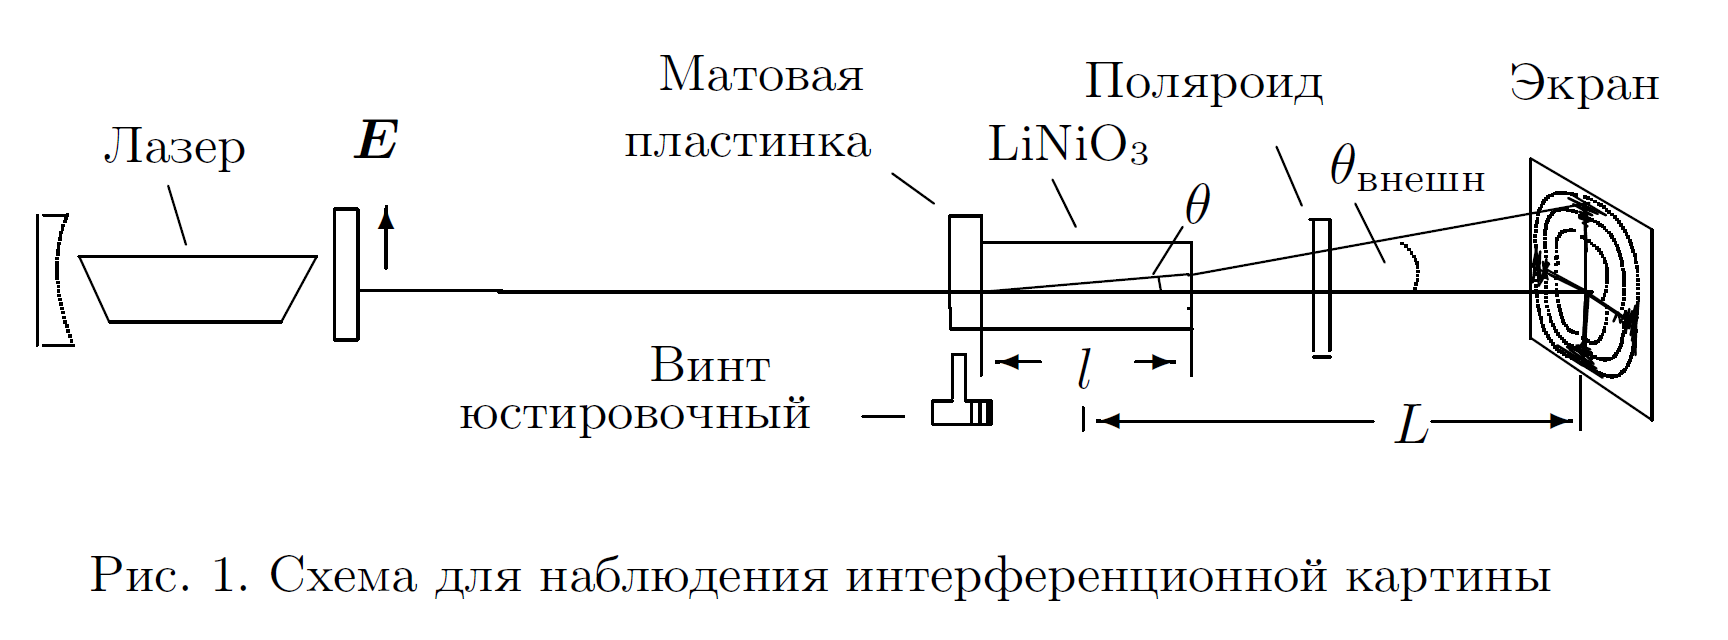
\includegraphics[width=0.9\textwidth]{th1.png}
	\label{fig:boiler}
\end{figure}

%Рассмотрим сначала кристалл в отсутствие внешнего электрического поля. Кристалл ниобата лития является одноосным кристаллом, то есть кристаллом, оптические свойства которого обладают симметрией вращения относительно некоторого одного направления, называемого оптической осъю $z$ кристалла. Для световой волны, вектор электрического поля $E$ которой перпендикулярен оси $z$, показатель преломления равен $n_o=\sqrt{\varepsilon_{\perp}}$, а для волны, вектор $E$ которой располагается вдоль оси $z$, он равен $n_e=\sqrt{\varepsilon_{\|}}$, причём $n_e<n_o$, т. е. $\mathrm{LiNbO}_3$ - «отрицательный кристалл».

В общем случае, когда луч света распространяется под углом $\theta$ к оптической оси $z$ (рис. 1 ), существуют два собственньх значения показателя преломления $n_1$ и $n_2$ : в обыкновенной волне (если световой вектор $E$ перпендикулярен плоскости $\left(k, e_z\right.$ ), где $k$ - волновой вектор луча, $e_z$ - орт по оси $z$ ) показатель $n_1=n_o$, а в необыкновенной (когда световой вектор $\boldsymbol{E}$ лежит в плоскости $\left(\boldsymbol{k}, \boldsymbol{e}_z\right)$ ) показатель преломления $n_2$ зависит от угла $\theta$ : согласно формуле (7.9), можем записать
$$
\frac{1}{n_2^2}=\frac{\cos ^2 \theta}{n_o^2}+\frac{\sin ^2 \theta}{n_e^2} .
$$

%Если перед кристаллом, помещённым между скрещенными поляроидами (рис. 1), расположить линзу или матовую пластинку, после которых лучи будут рассеиваться под различными углами, то на экране, расположенном за поляроидом, мы увидим тёмные концентрические окружности (коноскопическую картину) - результат интерференции обыкновенной и необыкновенной волн, точнее, проекцию их электрических полей на разрешённое направление выходного поляроида. В нашем эксперименте используется лазер, излучение которого поляризовано, поэтому входной поляроид можно не ставить.

Разность фаз между обыкновенной и необыкновенной волнами, приобретаемая при прохождении через кристалл длиной $\ell$, равна
$$
\Delta \varphi=\frac{2 \pi}{\lambda} \cdot \ell \cdot\left(n_1-n_2\right) .
$$

Для обыкновенного луча $n_1=n_o$ и не зависит от угла $\theta$ между направлением луча и осью $z$. Для необыкновенного луча $n_2$ зависит от угла $\theta$ и определяется уравнением (1). Считая, что $n_e$ и $n_o$ отличаются незначительно, для малых углов ( $\sin \theta \approx \theta, \cos \theta \approx 1-\theta^2 / 2$ ) полу чаем
$$
n_2 \approx n_o-\left(n_o-n_e\right) \theta^2 .
$$

Таким образом,

$$
\Delta \phi = \frac{2 \pi}{\lambda} l (n_0 - n_e) \theta^2 
$$

Направлениями постоянной разности фаз служат конусы $\theta = const$, поэтому интерференционная картина представляет собой концентрические окружности. Интерференционные кольца перерезаны тёмным "мальтийским крестом", который выделяет области, где интерференция отсутствует. В этих направлениях распространяется только одна поляризованная волна (обыкновенная или необыкновенная). При повороте выходного поляроида (анализатора) на 90$^\circ$ картина меняется с позитива на негатив: везде, где были светлые места, появляются тёмные и наоборот.

Для случая, когда разрешённое направление анализатора перпендикулярно поляризации лазерного излучения (скрещенные поляризации), найдём радиус тёмного кольца с номером $m$. Для луча, идущего вдоль оси $z(m=0)$, показатели преломления для двух волн совпадают, сдвиг фаз между ними равен нулю, поляризация излучения на вьходе остаётся такой же, как на входе, и луч не проходит через анализатор. Картина не изменится при сдвиге фаз между обыкновенной и необыкновенной волной, кратном $2 \pi$. Поэтому для $m$-го тёмного кольца $\Delta \varphi=2 \pi m$ или $\Delta \varphi=\frac{2 \pi}{\lambda} \ell\left(n_o-n_e\right) \theta^2=2 \pi m$. Если $L-$ расстояние от центра кристалла до экрана, то, учитывая закон преломления (закон Снеллиуса) на границе кристалла, при малых углах $\theta_{\text {внешн }}=n_o \theta$ (рис. 1) получаем выражение для радиуса кольца:
$$
r_m^2=\frac{\lambda}{\ell} \frac{\left(n_o L\right)^2}{\left(n_o-n_e\right)} m .
$$


\begin{figure}[!h]
	\centering
	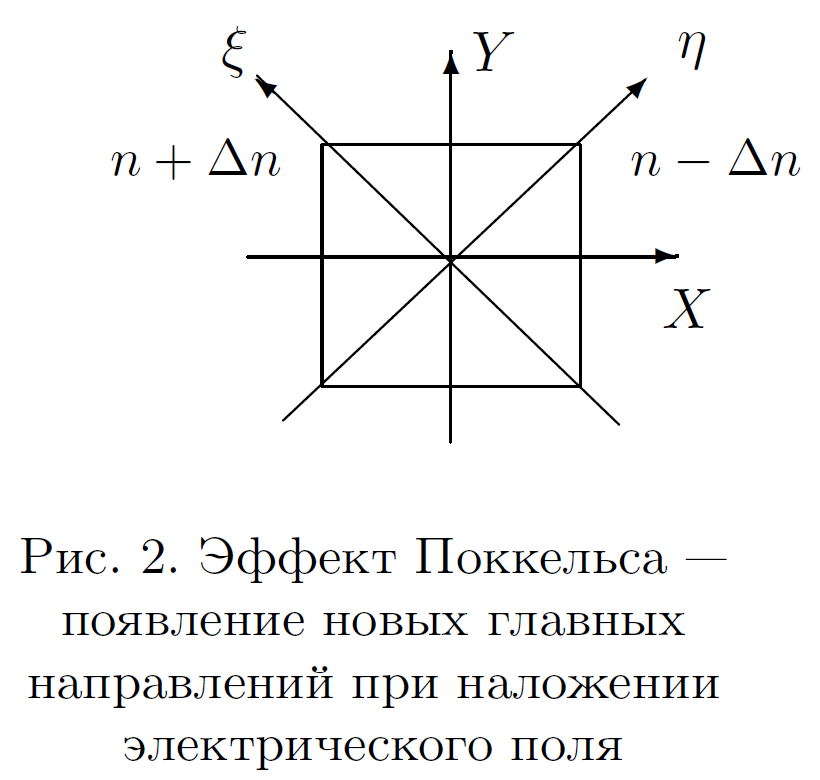
\includegraphics[width=0.5\textwidth]{th2.png}
	\label{fig:boiler}
\end{figure}




Измеряя радиусы колец, можно найти разность $\left(n_o-n_e\right)$ - двулучепреломление кристалла.

Представим теперь, что мы поместили кристалл в постоянное электрическое поле $E_{\text {эл }}$, направленное вдоль оси $x$, перпендикулярной оптической оси кристалла $z$. Луч света распространяется вдоль оси $z$, при этом для любой поляризации в отсутствие внешнего поля показатель преломления равен $n_o$. Свойства симметрии кристалла и его электрооптический тензор таковы, что в результате линейного электрооптического эффекта (эффекта Поккельса) в плоскости ( $x y$ ) возникают два главных направления $\xi$ и $\eta$ под углами $45^{\circ}$ к осям $x$ и $y$ (рис. 2) с показателями преломления $\left(n_o-\Delta n\right)$ и $\left(n_o+\Delta n\right.$ ), то есть появляются «медленная» и «быстрая» оси, причём $\Delta n=A \cdot E_{\text {эл }}$ ( $A$ - некая константа, зависящая только от типа кристалла).

Пусть свет на входе в кристалл поляризован вертикально, а на выходе стоит анализатор, пропускающий горизонтальную поляризацию. Разложим исходный световой вектор $E=E_0 e^{i(\omega t-k z)}$ по осям $\xi$ и $\eta$ : $E_{\xi}=E_\eta=E_0 / \sqrt{2}$. После прохождения кристалла между векторами $E_{\xi}$ и $E_\eta$ появится разность фаз:
$$
\Delta \varphi=\frac{2 \pi \ell}{\lambda} 2 \Delta n=\frac{4 \pi \ell}{\lambda} A E_{\text {эл }}=\frac{4 \pi}{\lambda} \frac{\ell}{d} A U,
$$

где $U=E_{\text {эл }} d$ - напряжение на кристалле, $d-$ размер кристалла в поперечном направлении. Результирующее поле после анализатора это сумма проекций $E_{\xi}$ и $E_\eta$ на направление $x$, т. е.
$$
E_{\text {вых }}=\frac{E_0}{2} e^{i(\omega t-k \ell)}\left(e^{i \Delta \varphi / 2}-e^{-i \Delta \varphi / 2}\right)=E_0 e^{i(\omega t-k \ell)} \sin \left(\frac{\Delta \varphi}{2}\right) .
$$

Интенсивность света пропорциональна квадрату модуля вектора электрического поля в волне:
$$
I_{\text {вых }} \sim E E^*=E_0^2 \sin ^2\left(\frac{\Delta \varphi}{2}\right),
$$

поэтому
$$
I_{\text {вых }}=I_0 \sin ^2\left(\frac{\Delta \varphi}{2}\right)=I_0 \sin ^2\left(\frac{\pi}{2} \frac{U}{U_{\lambda / 2}}\right) .
$$

Здесь
$$
U_{\lambda / 2}=\frac{\lambda}{4 A} \frac{d}{\ell}
$$
- так называемое полуволновое напряжение - имеет тот смысл, что при $U=U_{\lambda / 2}$ сдвиг фаз между двумя волнами, соответствующими двум собственным поляризациям, $\Delta \varphi=\pi$ (разность хода равна $\lambda / 2$ ), и интенсивность света на выходе анализатора, как следует из (3), достигает максимума.

В работе предлагается показать, что при параллельных поляризациях лазера и анализатора
$$
I_{\text {вых }}=I_0 \cos ^2\left(\frac{\pi}{2} \frac{U}{U_{\lambda / 2}}\right) .
$$

Напряжение $U_{\lambda / 2}$ называют также управляющим напряжением. Оно уменьшается, как это видно из (4), с уменьшением длины волны света $\lambda$ и с увеличением отношения $\lambda / d$ кристалла (это справедливо для поперечного электрооптического эффекта, который используется в нашем опыте). Характерная величина полуволнового напряжения в ниобате лития для видимого света составляет несколько сотен вольт.

\section{Экспериментальная установка}

\begin{figure}[!h]
	\centering
	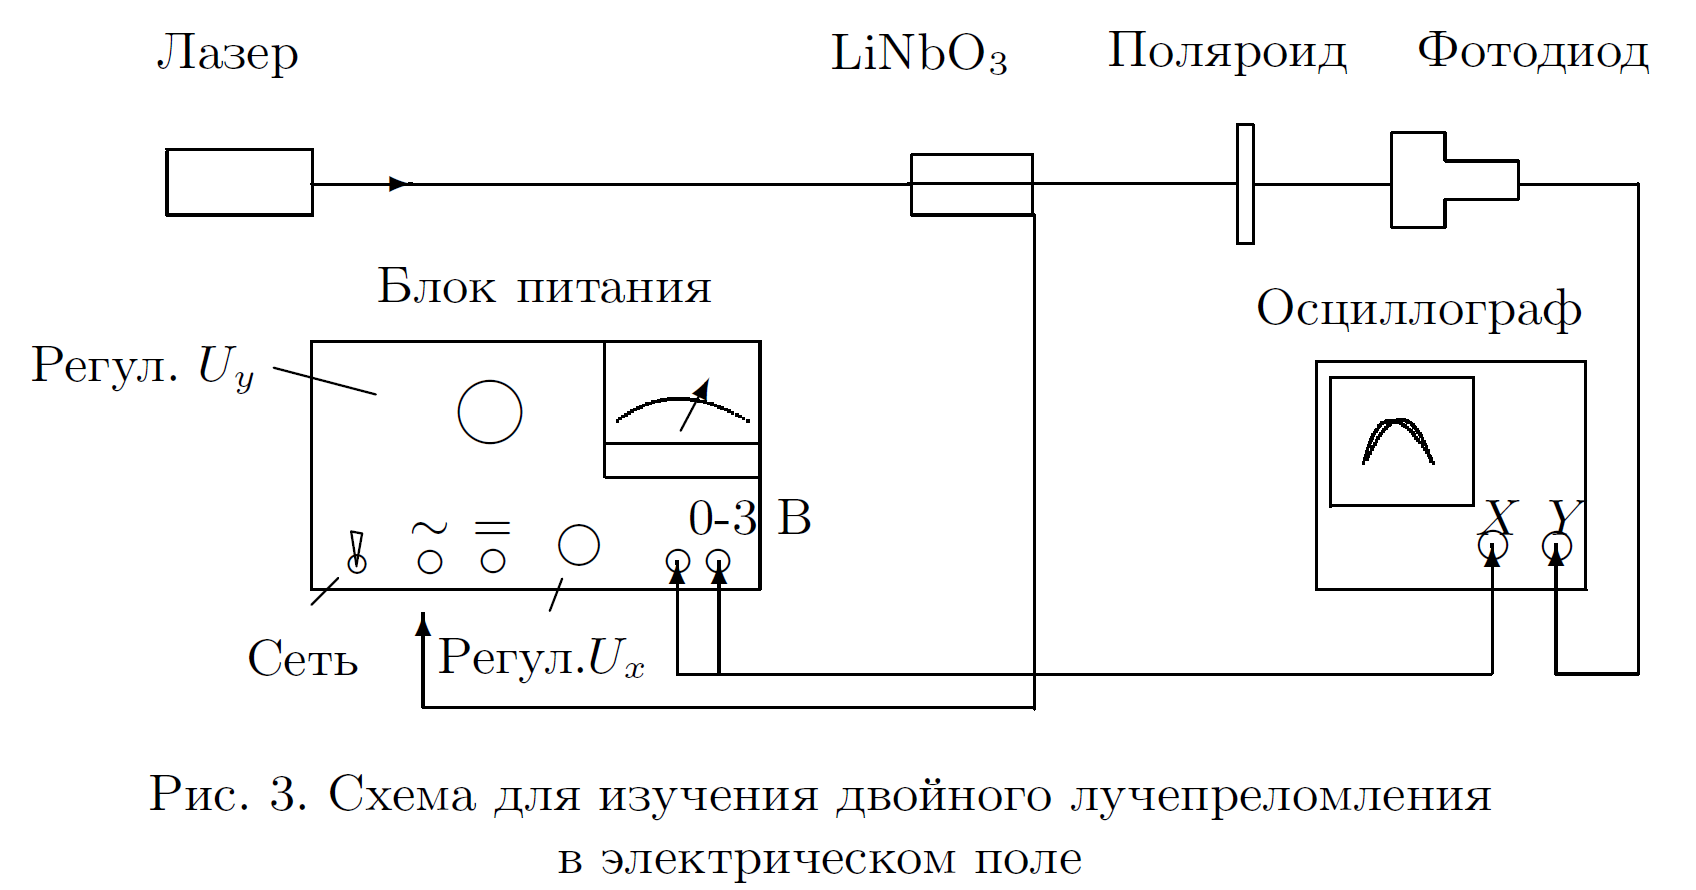
\includegraphics[width=0.9\textwidth]{установка.png}
	\label{fig:boiler}
\end{figure}

Свет гелий-неонового лазера, поляризованный в вертикальной плоскости, проходя сквозь матовую пластинку, рассеивается и падает на двоякопреломляющий кристалл под различными углами. Кристалл ниобата лития с размерами 3×3×26 мм вырезан вдоль оптической оси $z$. На экране, расположенном за скрещенным поляроидом, видна интерференционная картина.

Для $\lambda = 0.63$ мкм (длина волны гелий-неонового лазера) в ниобате лития $n_0 = 2.29$.

Убрав рассеивающую пластинку и подавая на кристалл постоянное напряжение, можно величиной напряжения влиять на поляризацию луча, вышедшего из кристалла.

Заменив экран фотодиодом (рис. 3) и подав на кристалл переменное напряжение, можно исследовать поляризацию луча с помощью осциллографа.

\section{Измерения, Обработка}

1) Предварительно отъюстируем систему, хотя в процессе эксперимента это все равно придется неоднократно повторить. Убедимся в том, что лазерный луч поляризован вертикально, а у поляроида найдем вертикальное разрешённое направление.

2-3) Расположим интерференционную картину со сдвигом, чтобы наблюдать наибольшее количество колец.

Расстояние $L = 74.0 \pm 0.5$ см.

Длина волны излучения гелий-неонного лазера $\lambda = 0.63$ мкм.

Показатель преломления кристалла $n_0 = 2.29$

Длина кристалла $l = 26$ мм.

4) Данные приведены в таблице

\begin{center}
	\Large Зависимость радиуса кольца от его номера
\end{center}

\begin{center}
\begin{tabular}{|c|c|}
\hline 
n & $r$, см \\
\hline 
1 &	2.6 \\
2 &	3.6 \\
3 &	4.5 \\
4 &	5.1 \\
5 &	5.8 \\
6 &	6.3 \\
7 &	7.3 \\
8 &	7.7 \\
9 &	8.2 \\
\hline

\hline
\end{tabular}
\end{center}

\begin{center}
	\Large Зависимость $r^2(n)$
\end{center}

\begin{figure}[!h]
	\centering
	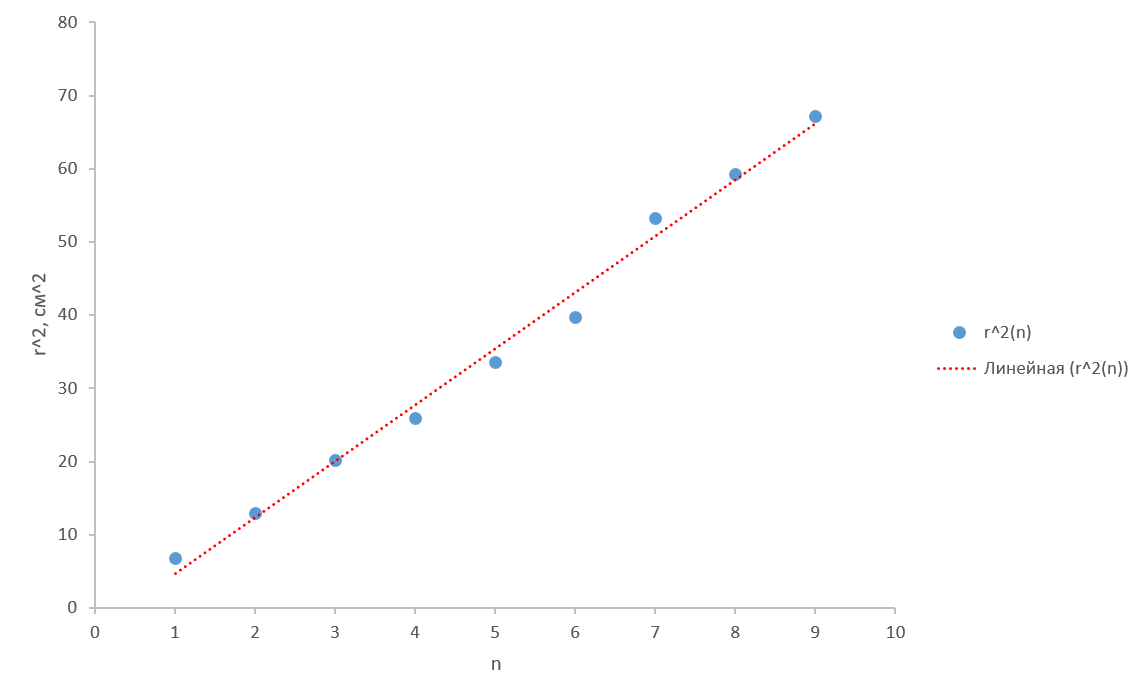
\includegraphics[width=0.9\textwidth]{граф1.png}
	\label{fig:boiler}
\end{figure}

Найдем угловые коэффициенты прямых для каждой установки по МНК.

\[
	a = \frac{<x_i y_i> - < x > < y_i >}{< x_i^2> - < x_i >^2}
\]

\[
	b = < \nu_i > - a < N_i >
\]

Также рассчитаем их погрешности

\begin{equation}
	S_a^2 = \frac{< x_i^2>}{< x_i^2 > - < x_i >^2} \cdot \frac{<  b_i - b > ^2}{n - 2}
\end{equation}

Итоговая зависимость

$$r^2 = (-2.9 \pm 1.5) + (7.68 \pm 0.27) \cdot m$$

\begin{equation}
	n_0 - n_e = 0.091 \pm 0.005
\end{equation}

Это совпадает с табличным значением 0.09 в пределах погрешности.

5) Уберем матовую пластинку и отъюстируем систему.

Включим ЛБП в сеть и убедимся в работоспособности установки.

Удобнее всего проводить замеры при исходной параллельной поляризации, тогда полуволновому напряжению будет соответствовать минимум яркости.

Полученное значение

\begin{equation}
	U_{\lambda / 2} = 450 \text{ В}
\end{equation}

6) При четвертьволновом напряжении $U_{\lambda / 2}$ получается круговая поляризация, т.е. интенсивность не меняется при вращении поляроида.

7) Проведем наблюдения с помощью фотодиода и осциллографа, расположим фотодиод на расстоянии около 40-50 см от кристалла, чтобы минимизировать вклад рассеянного излучения лазера и максимизировать попадающее на элемент излучение центрального луча.

8-9) Занесу в таблицу результаты измерения напряжений по фигурам Лиссажу и визуально

\begin{center}
\begin{tabular}{|c|c|c|c|}
\hline 
& $U_{\lambda / 2}$, В & $U_{\lambda}$, В & $U_{3 \lambda / 2}$, В\\
\hline 
Лиссажу & 420 & 840 & 1260 \\
Визуал  & 450 & - & - \\
\hline

\end{tabular}
\end{center}

Результаты сходятся в рамках возможных неточностей.

\begin{figure}[!h]
	\centering
	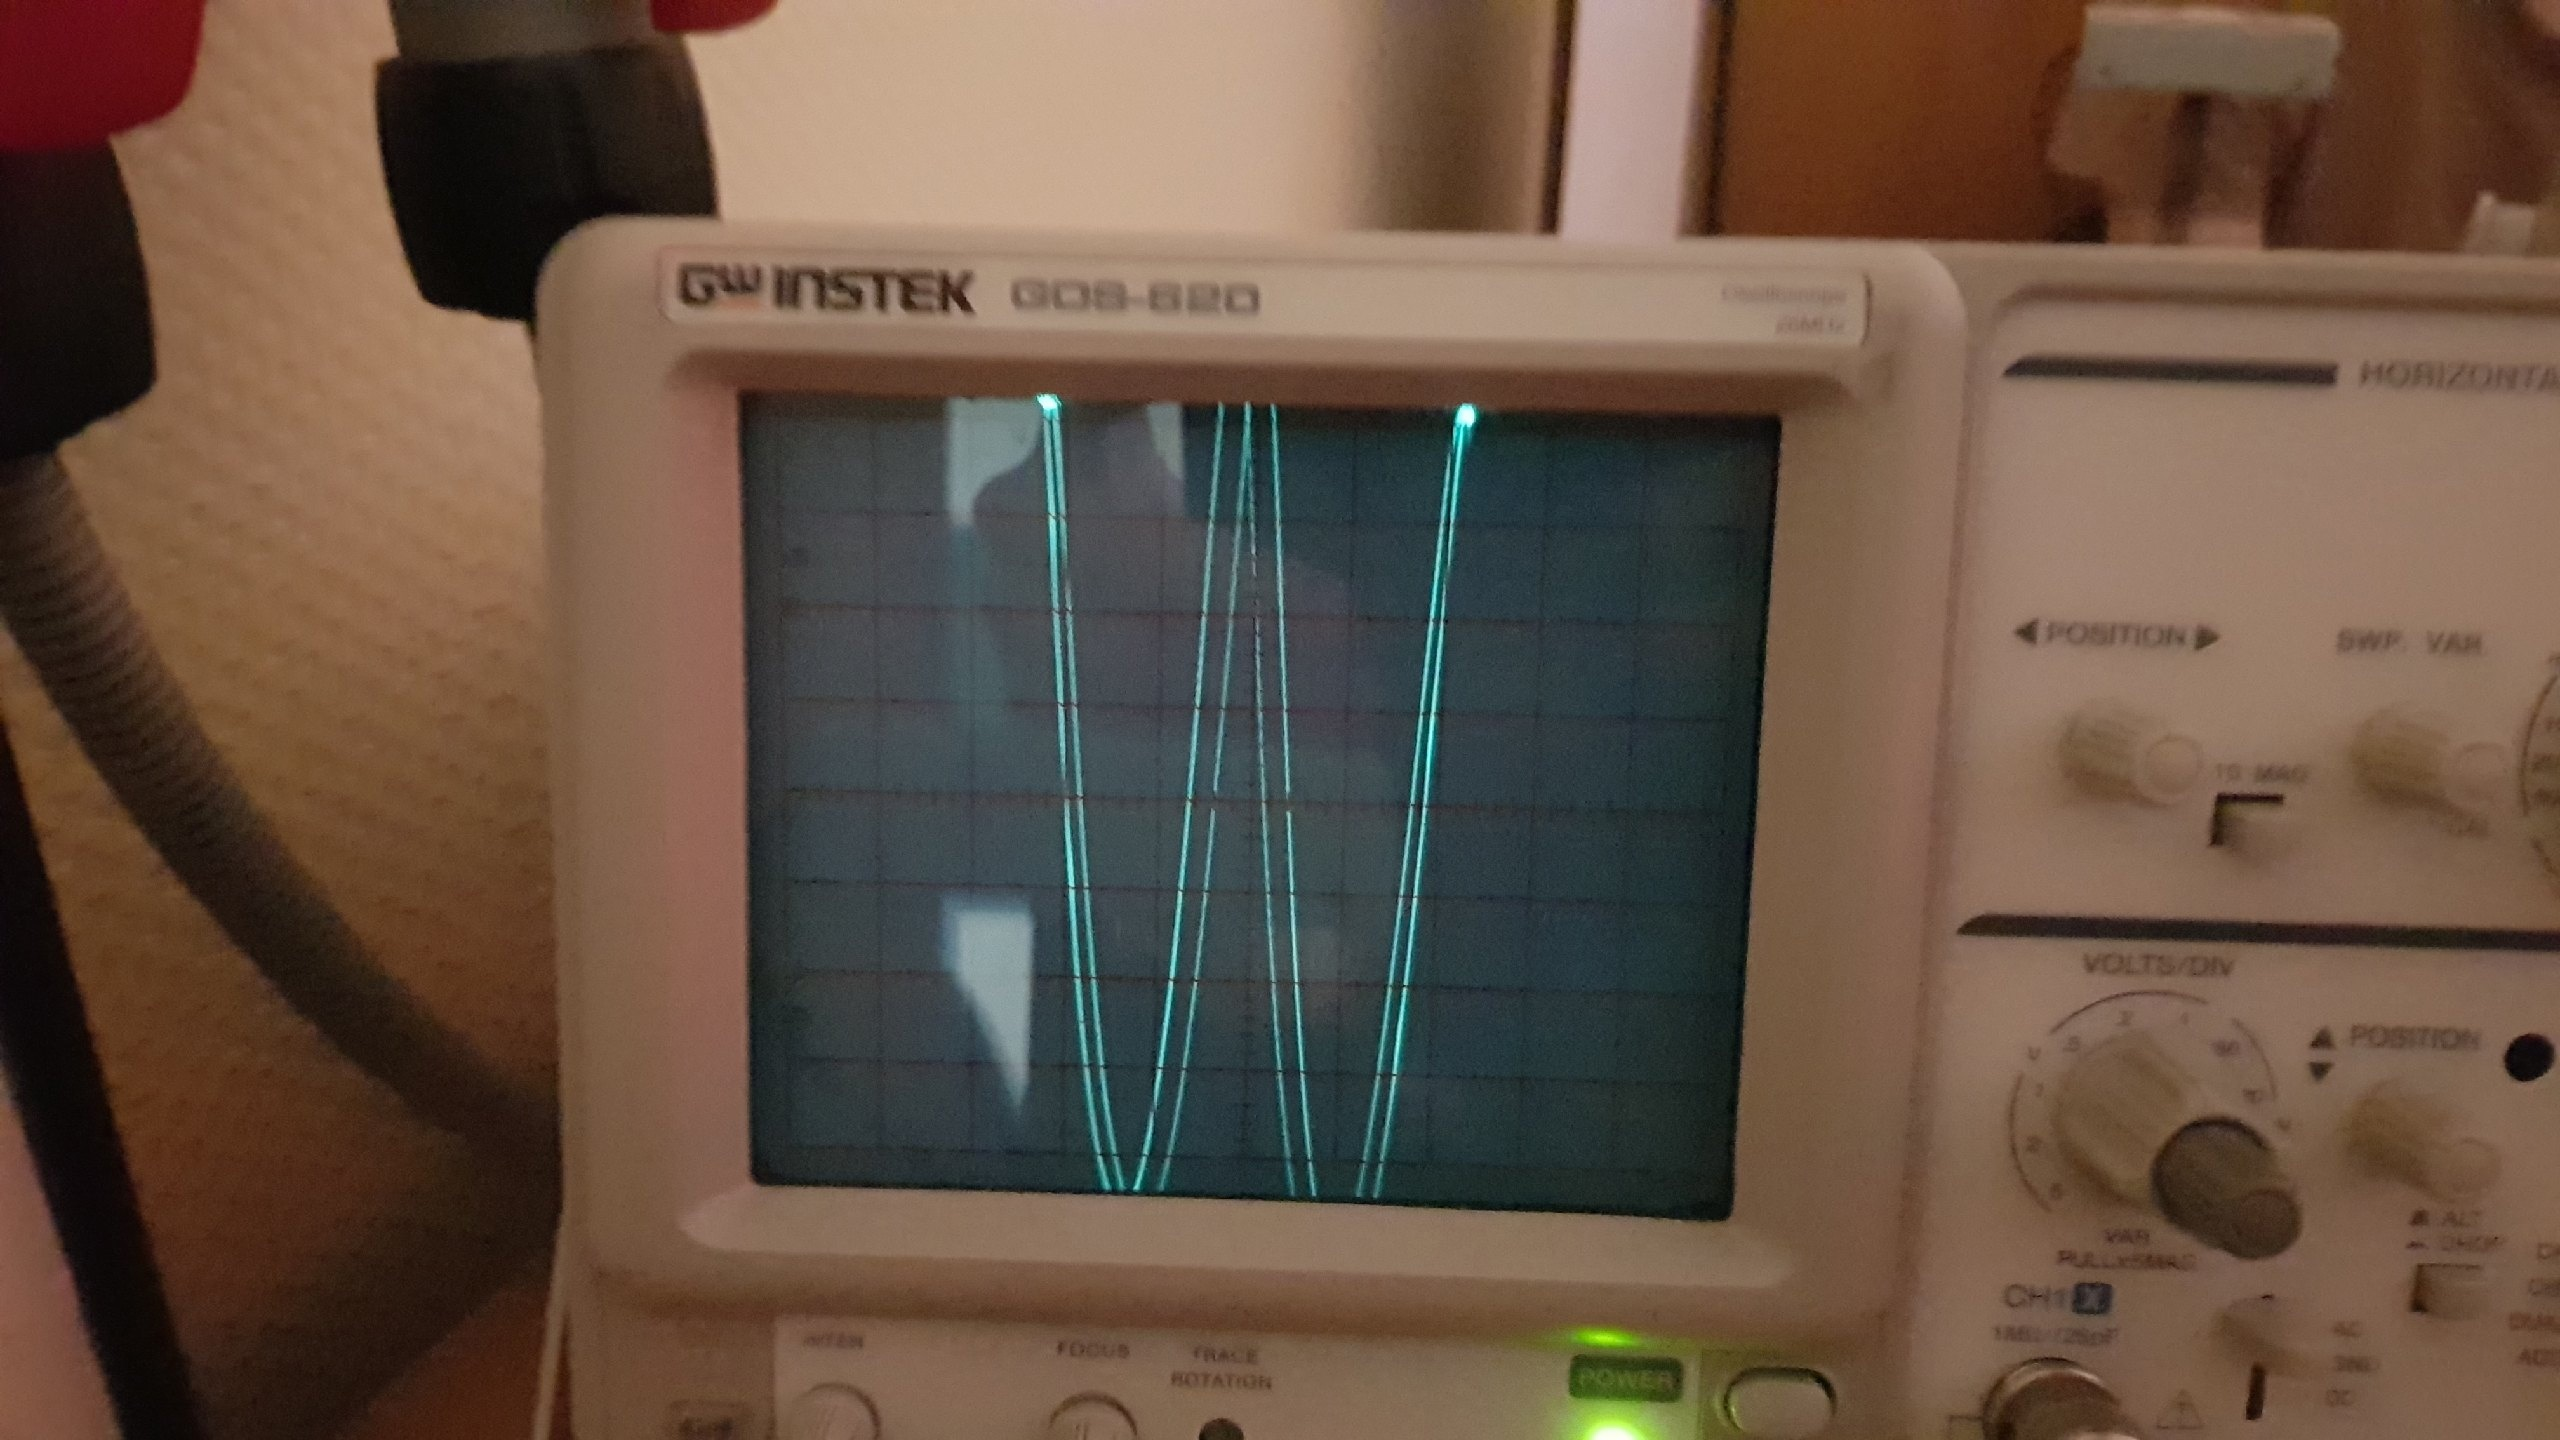
\includegraphics[width=0.9\textwidth]{1jErPQcC5tQ.jpg}
	\label{fig:boiler}
	\caption{Полуволновое}
\end{figure}

\begin{figure}[!h]
	\centering
	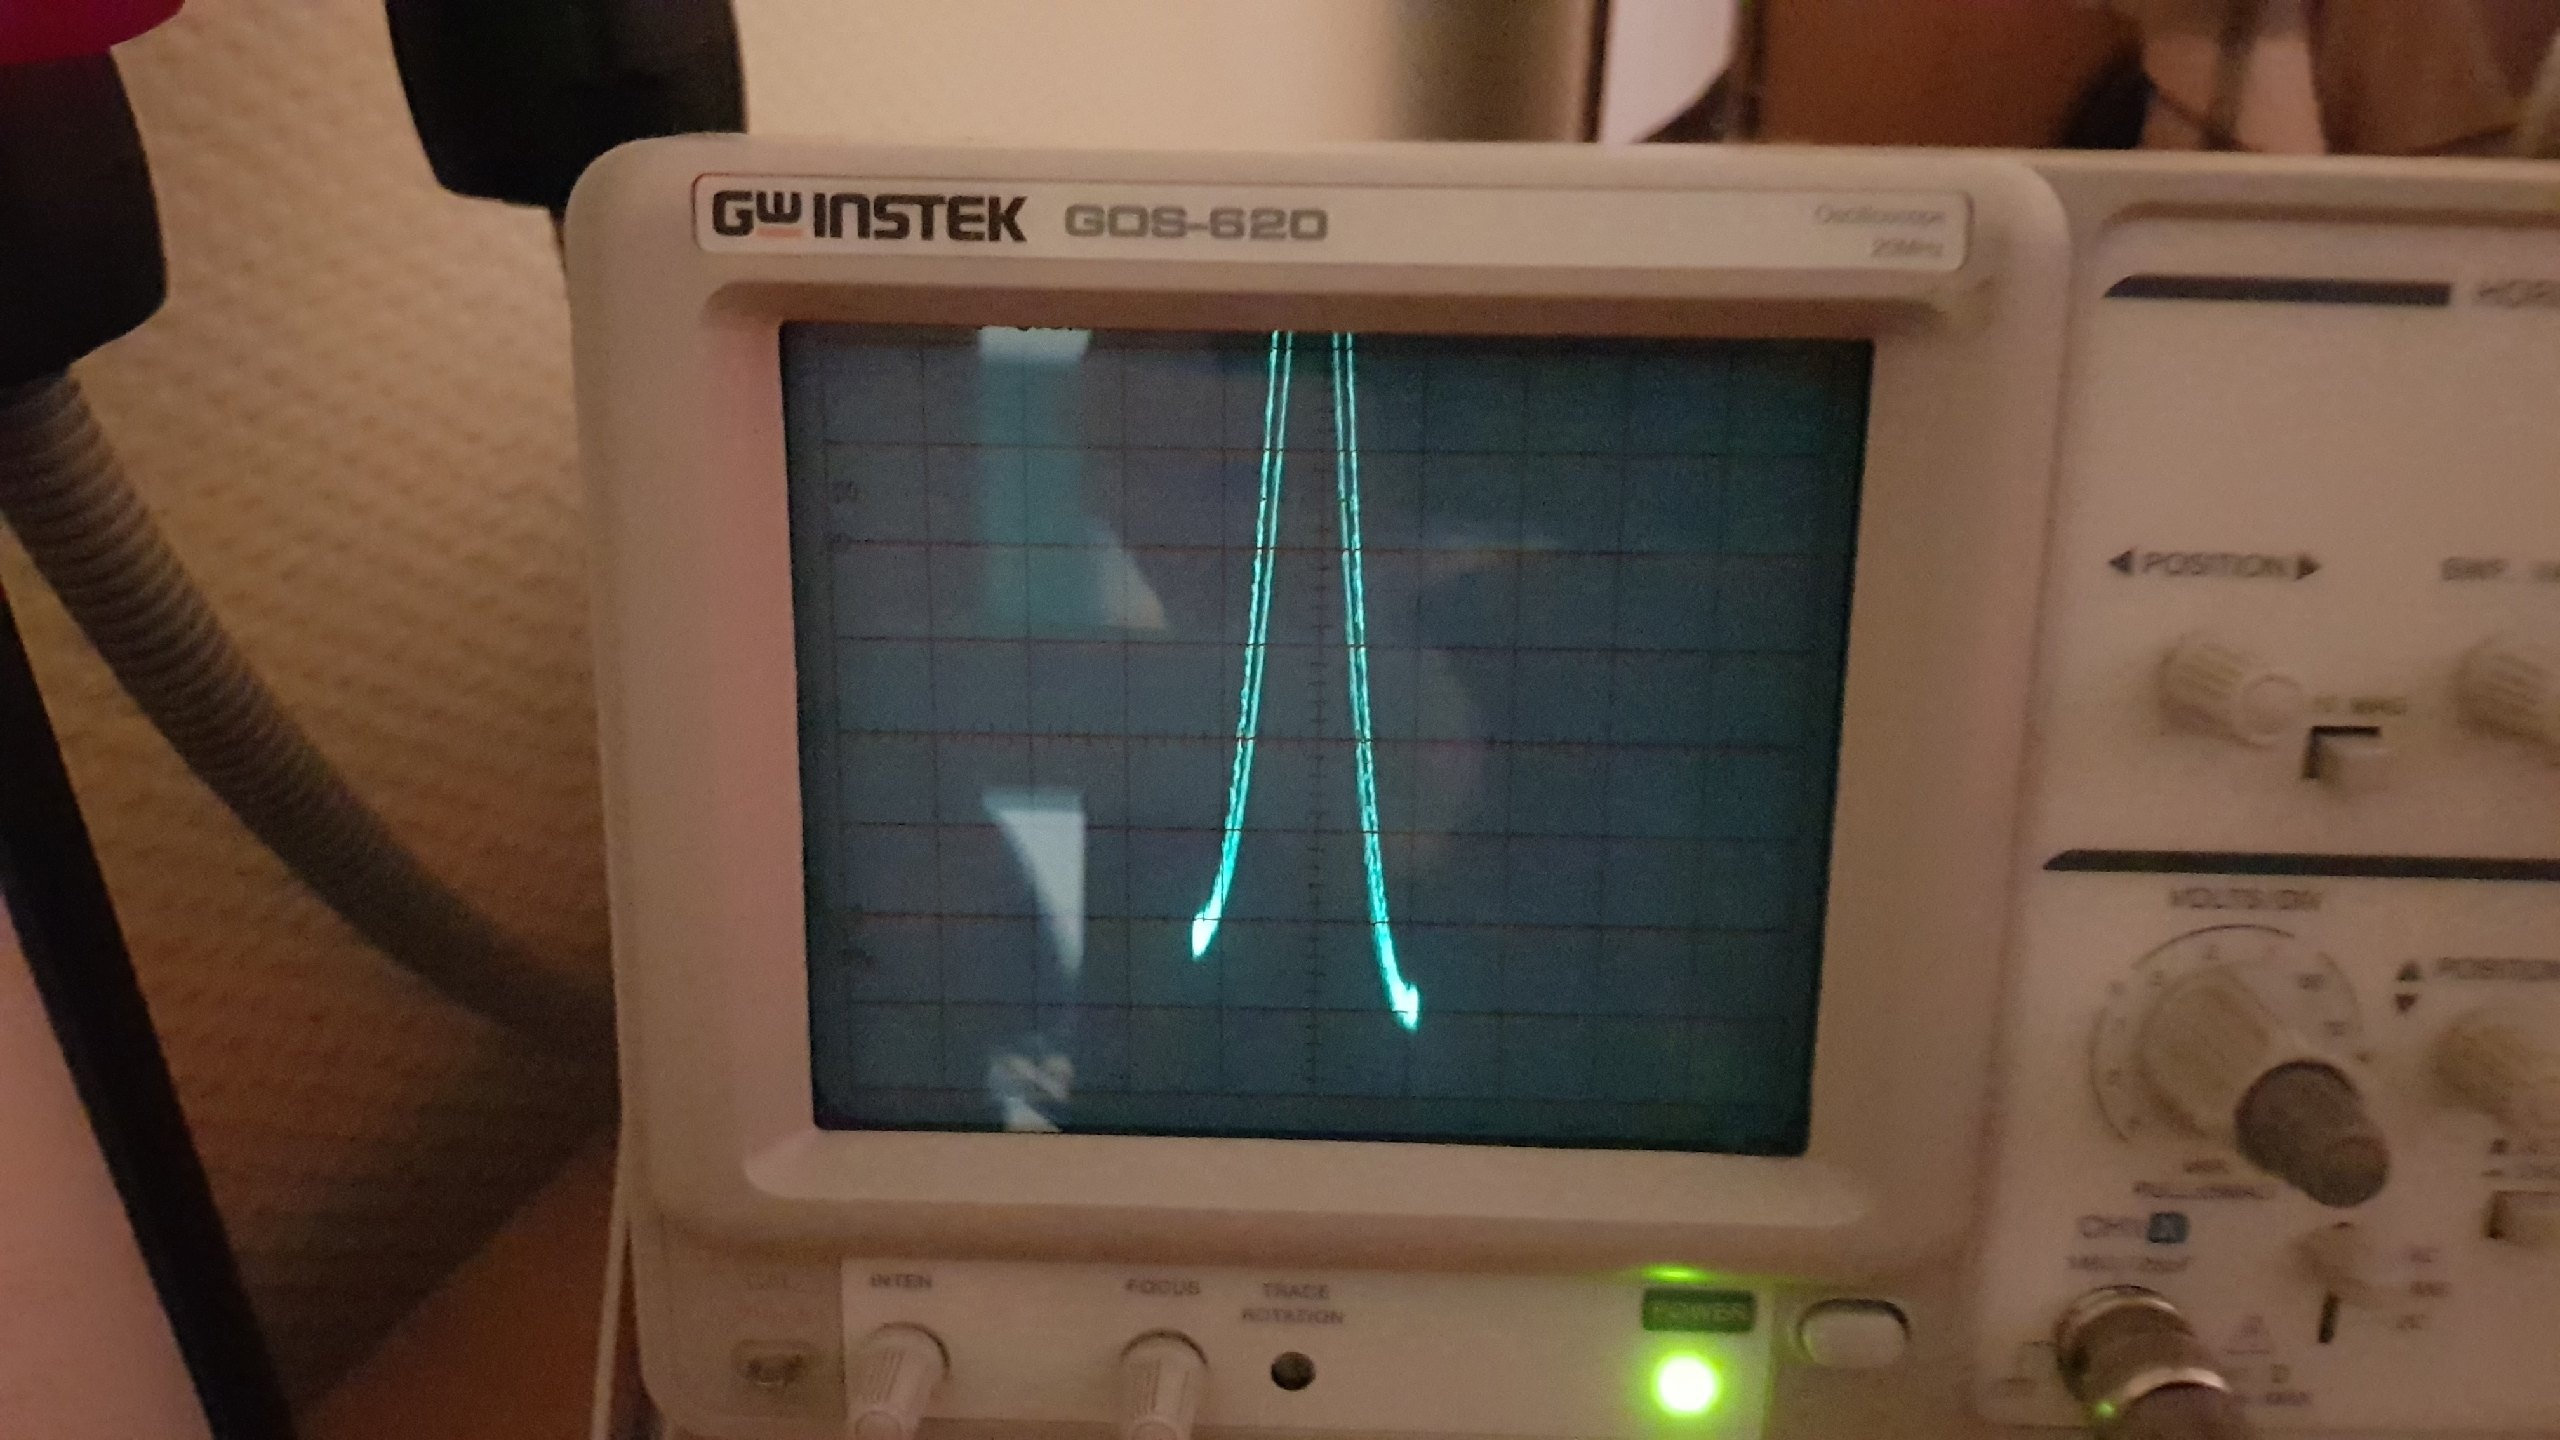
\includegraphics[width=0.9\textwidth]{wKRP0k59XyQ.jpg}
	\label{fig:boiler}
	\caption{Волновое}
\end{figure}

\newpage
.
\begin{figure}[!h]
	\centering
	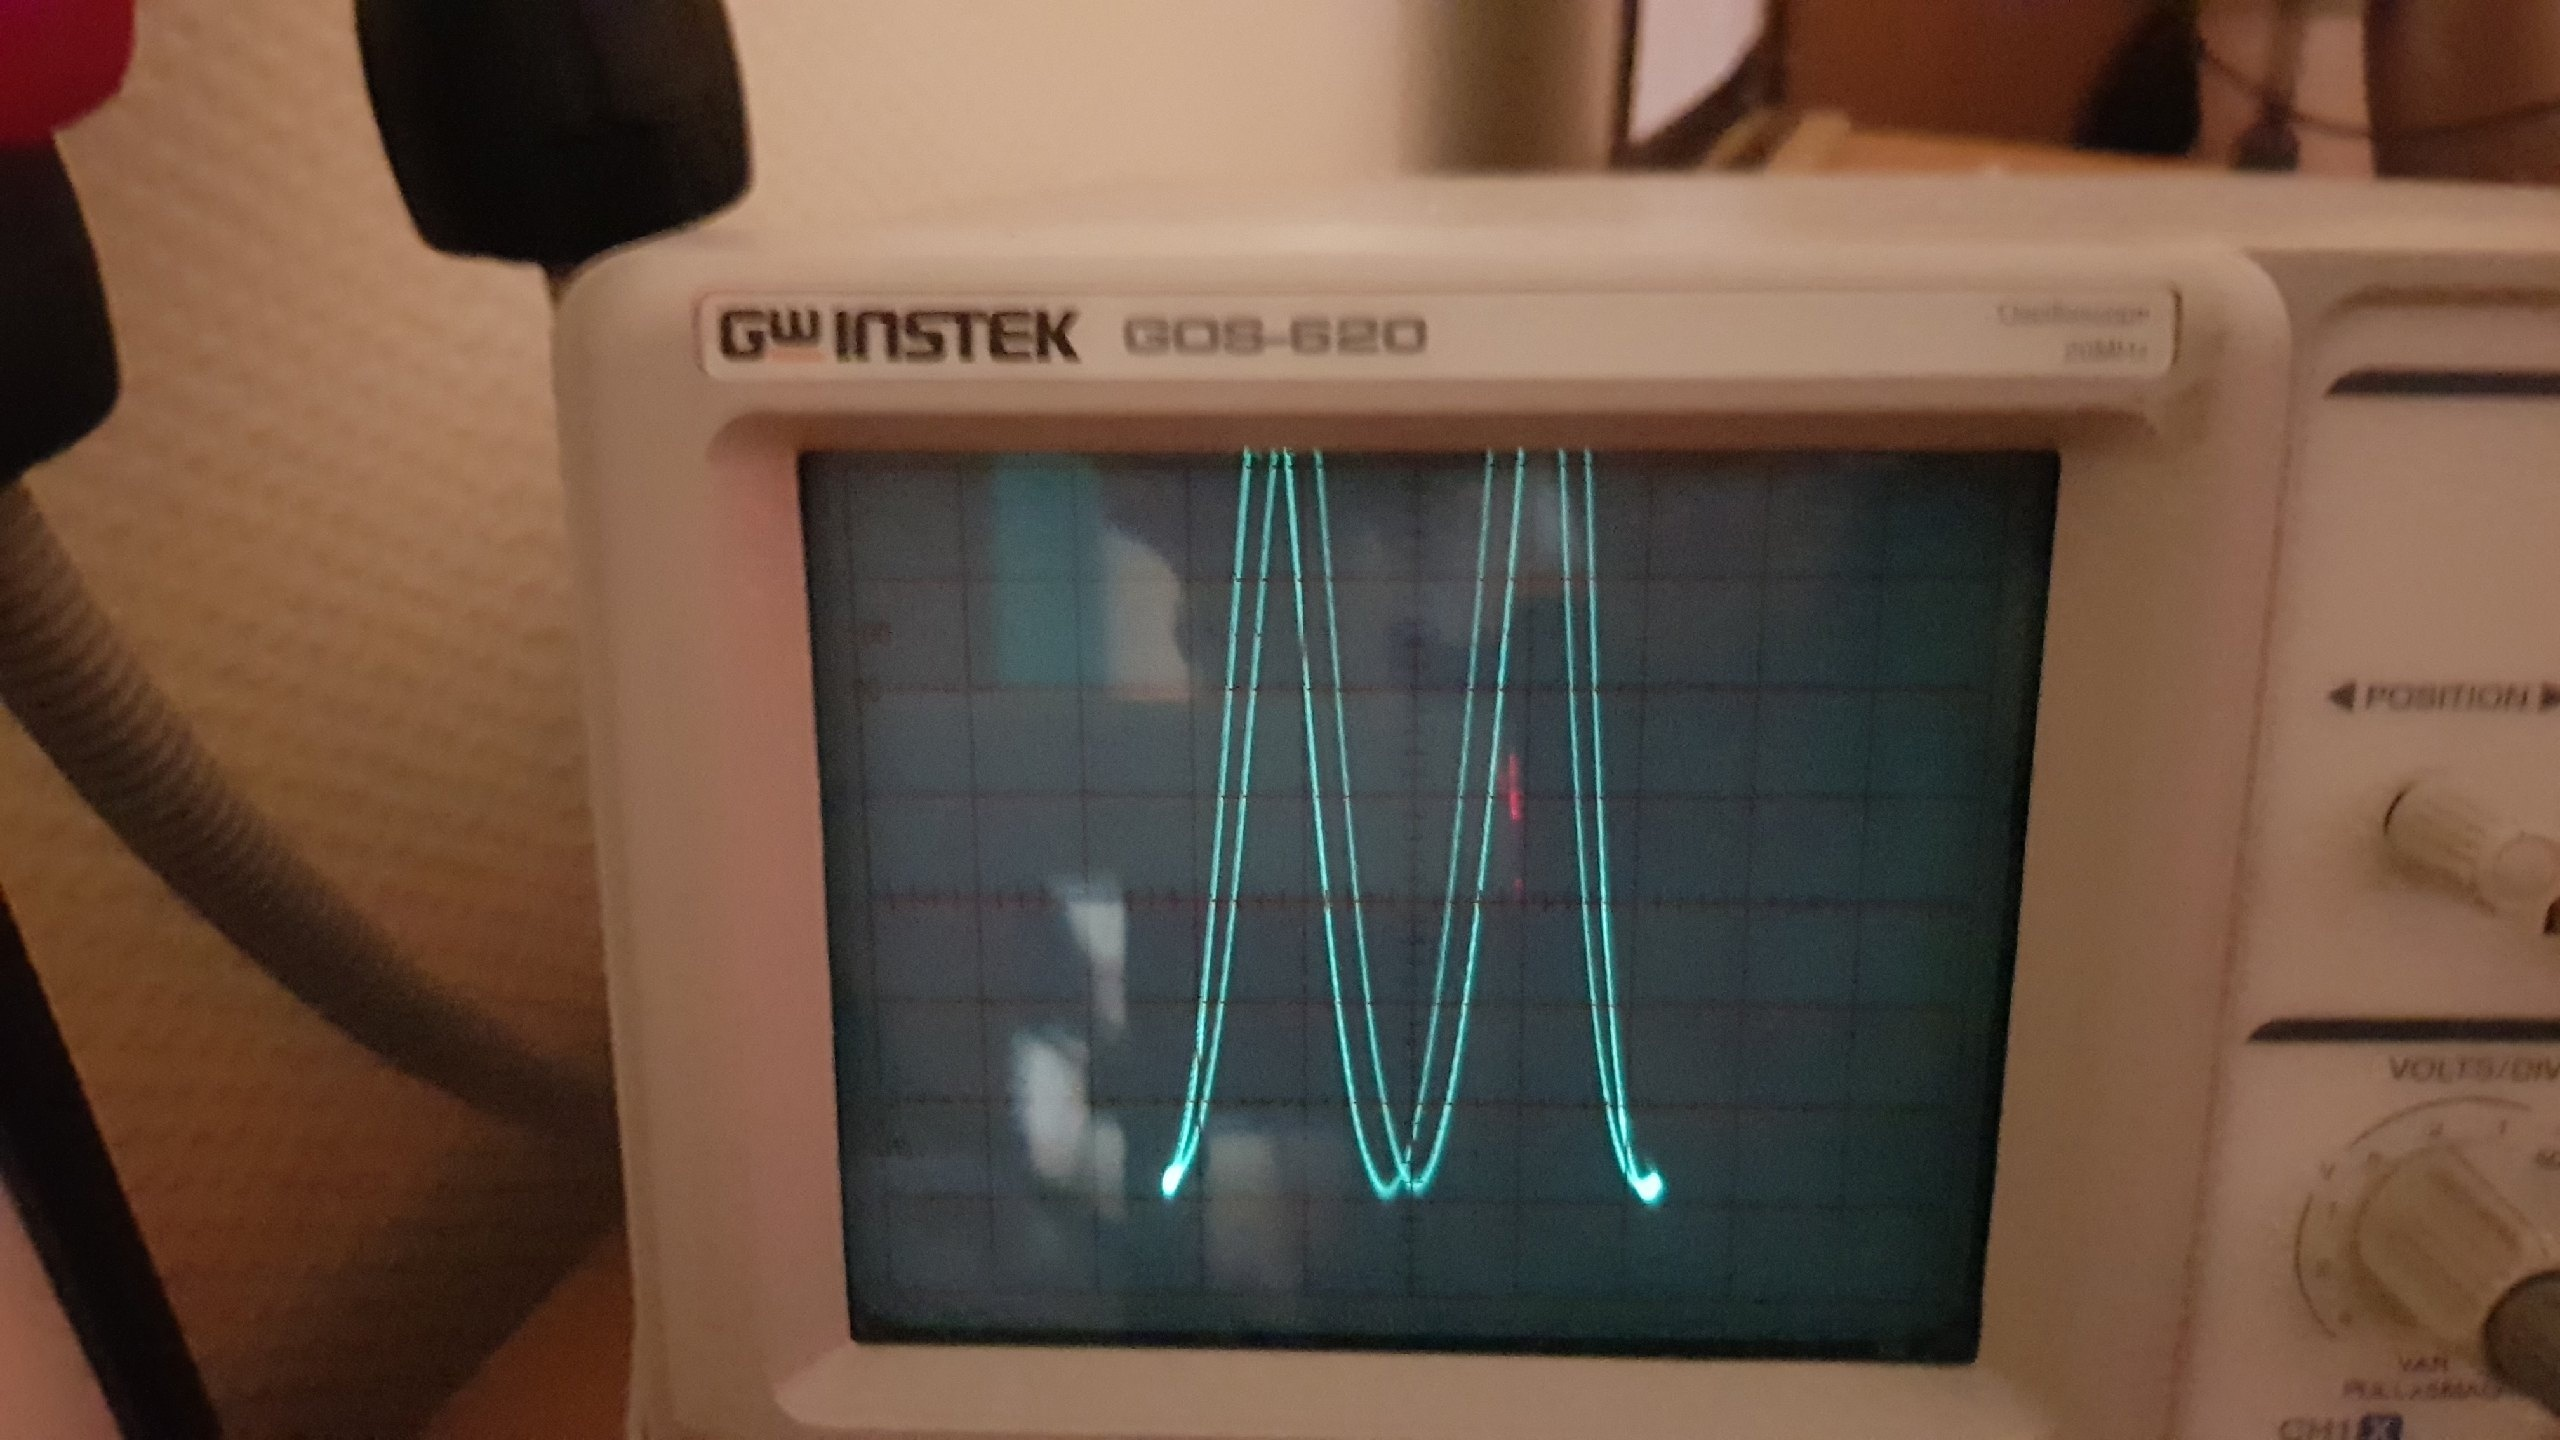
\includegraphics[width=0.9\textwidth]{YST5G-3Lncg.jpg}
	\label{fig:boiler}
	\caption{Волновое инвертированное}
\end{figure}

\newpage

\section{Вывод}

Были проведены замеры как двулучепреломления на основе интерференционной картины поляризованного света, прошедшего через кристалл, так и волновых напряжений, соответствующих своим фигурам Лиссажу. Результаты совпали с табличными, что свидетельствует о верной постановке эксперимента и грамотно заданных приближениях.

\section{Ресурсы}

Расчет по МНК: метод-наименьших-квадратов.рф


\end{problem}
\end{document}